
\documentclass[12pt, a4paper]{article}
\usepackage{graphicx}
\usepackage{amsmath}
\usepackage{float}
\usepackage{listings}
\usepackage{lmodern}  % for bold teletype font
\usepackage{xcolor}   % for \textcolor



\title{\textbf{EE2703 : Applied Programming Lab \\ Assignment 4}} % Title

\author{Potta Muni Asheesh \\ EE19B048} % Author name

\date{\today} % Date for the report

\begin{document}	
\lstset{
  language=Python,
  basicstyle=\ttfamily,
  columns=fullflexible,
  frame=single,
  breaklines=true,
  postbreak=\mbox{\textcolor{red}{$\hookrightarrow$}\space},
}	
		
\maketitle % Insert the title, author and date
\section{Aim}
 We will be fitting two functions, namely, $exp(x)$ and $cos(cos(x))$ over an interval of [0, $2\pi$) using Fourier series.
 \begin{equation*}
 	a_0 + \sum_{n=1}^{\infty}(a_{n}cos(nx)+b_{n}sin(nx))
 \end{equation*}
 The coefficients $a_0, a_{n}, b_{n}$ are given by
 \begin{align*}
 	a_0 &= \frac{1}{2\pi} \int_{0}^{2\pi}f(x)dx \\
 	a_n &= \frac{1}{\pi} \int_{0}^{2\pi}f(x)cos(nx)dx \\
 	b_n &= \frac{1}{\pi} \int_{0}^{2\pi}f(x)sin(nx)dx
 \end{align*}  
 
\section{Assignment questions}

\subsection{Plotting the two functions}
	We can define functions which use functions from \texttt{numpy} to compute the required function for a given vector(or scalar) and returns a vector(or scalar). The functions are named as \texttt{e} and \texttt{coscos} in the code.
\begin{lstlisting}
def e(x):
    return np.exp(x)

def coscos(x):
    return np.cos(np.cos(x))	
\end{lstlisting}
	The plot of these two functions over the interval $[-2\pi, 4\pi)$ is given below.\\
	It is seen that $cos(cos(x))$ is periodic and $exp(x)$ is not periodic. When we compute the Fourier series of these two functions, the generated function is expected to be over the interval $[0, 2\pi)$, as shown below
	\begin{figure}[H]
		\centering
		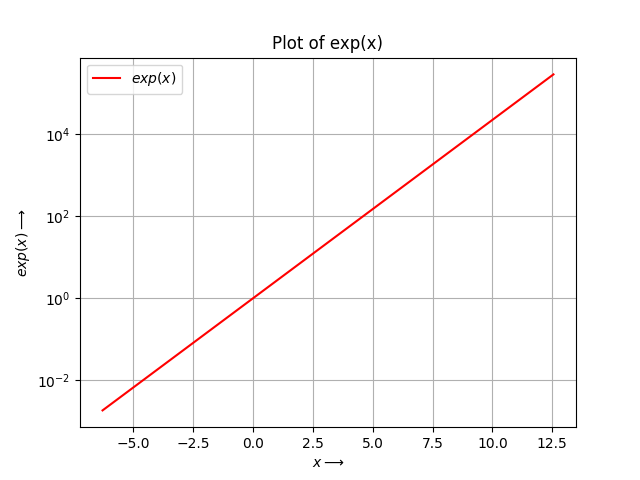
\includegraphics[scale=0.75]{Figure_1.png}
		\caption{Plot of $exp(x)$ (semi-log scale)}
		\centering
		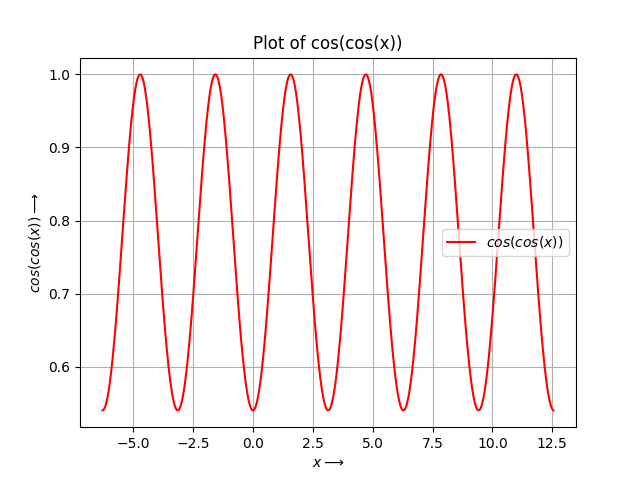
\includegraphics[scale=0.75]{Figure_2.png}
		\caption{Plot of $cos(cos(x))$}
	\end{figure}
	\begin{figure}[H]
		\centering
		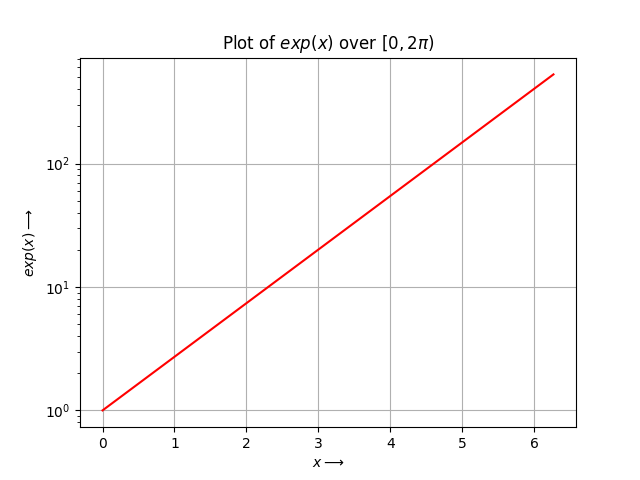
\includegraphics[scale=0.75]{Figure_13.png}
		\caption{Plot of $exp(x)$}
		\centering
		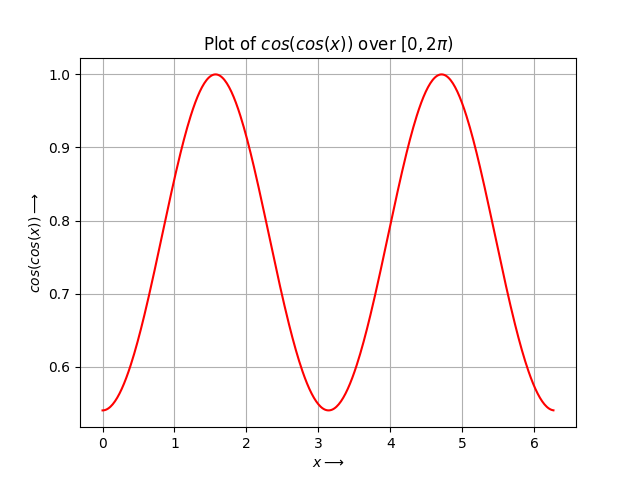
\includegraphics[scale=0.75]{Figure_14.png}
		\caption{Plot of $cos(cos(x))$}
	\end{figure}
	
\subsection{Obtaining Fourier coefficients using direct integration}
	As discussed above, we can use integration to find the coefficients of the Fourier series. In Python, we can do definite integration using \texttt{quad} function from \texttt{scipy.integrate}. Two Python functions \texttt{u(x, k, f) = f(x)cos(kx)} and \texttt{v(x, k, f) = f(x)sin(kx)} are defined, to pass to \texttt{quad} function, as shown below
\begin{lstlisting}
def u(x, k, f):
    return f(x)*np.cos(k*x)

def v(x, k, f):
    return f(x)*np.sin(k*x)
\end{lstlisting}
	Here, the parameter \texttt{f} should be a function and it should return a scalar or vector. The functions defined previously are used here. \texttt{for} loop is used to find the coefficients iteratively as shown below. The coefficients for $exp(x)$ and $cos(cos(x))$ are stored in arrays named \texttt{coeffs\_f1} and \texttt{coeffs\_f2} respectively.
\begin{lstlisting}
coeffs_f1 = np.zeros(51)
coeffs_f2 = np.zeros(51)
coeffs_f1[0] = quad(u, 0, 2*pi, args=(0,e))[0]/(2*pi)
coeffs_f2[0] = quad(u, 0, 2*pi, args=(0,coscos))[0]/(2*pi)

for i in range(1, 26):
    coeffs_f1[2*i-1] = quad(u, 0, 2*pi, args=(i,e))[0]/pi
    coeffs_f1[2*i] = quad(v, 0, 2*pi, args=(i,e))[0]/pi
    coeffs_f2[2*i-1] = quad(u, 0, 2*pi, args=(i,coscos))[0]/pi
    coeffs_f2[2*i] = quad(v, 0, 2*pi, args=(i,coscos))[0]/pi
\end{lstlisting}
 
\subsection{Plotting the coefficients}
To plot the 51 coefficients, they are first arranged in a vector as shown below.
$$\begin{pmatrix}
	a_0 \\
	a_1 \\
	b_1 \\
	... \\
	a_{25} \\
	b_{25} \\
\end{pmatrix}$$ 
Now, this vector is plotted against $n$ as $n$ varies from 1 to 51. For each set of the coefficients, two plots are made, one with \textit{log} scale on y-axis only and the other with \textit{log} scale on both x and y axes. The plots of absolute values of the coefficients are shown below.\\ 
It is found that $b_n$ for the function $cos(cos(x))$ are of the order $10^{-15}-10^{-17}$ which for practical purposes can be approximated to $0$.  This happens because $cos(cos(x))$ is an even function and coefficients of $sin$ terms in Fourier series are 0 for even functions.

The coefficients for $exp(x)$ are given as
\begin{align*}
a_n &= \frac{e^{2\pi} - 1}{\pi(1 + n^2)} \\
b_n &= \frac{-n(e^{2\pi} - 1)}{\pi(1 + n^2)}
\end{align*}
So, they decay as $\sim \frac{1}{n^2}$ and $\sim \frac{1}{n}$ which is not as quick as the coefficients of $cos(cos(x))$. This is because, as $exp(x)$ is not periodic, higher frequency sinusoids are also required for good enough convergence. They look linear in the \textit{loglog} plot because they decay as shown above. The coefficients of $cos(cos(x))$ are related to Bessel functions as they can be evaluated from the integral form of Bessels functions, so they look linear in semi-log-y plot.
\begin{figure}[H]
\centering
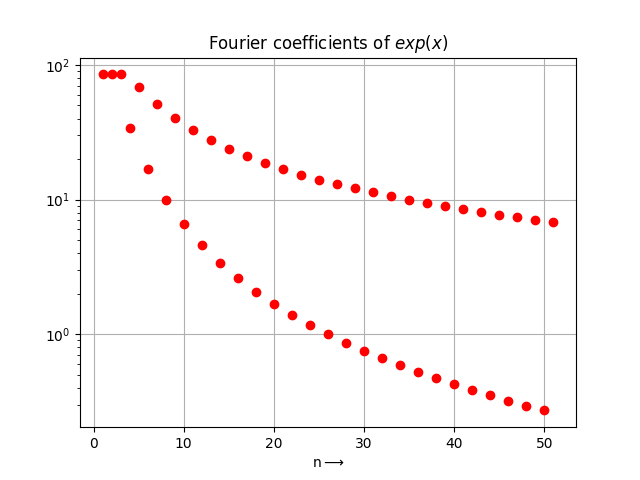
\includegraphics[scale=0.75]{Figure_9.png}
\caption{Coefficients for $exp(x)$ (semilogy)}
\centering
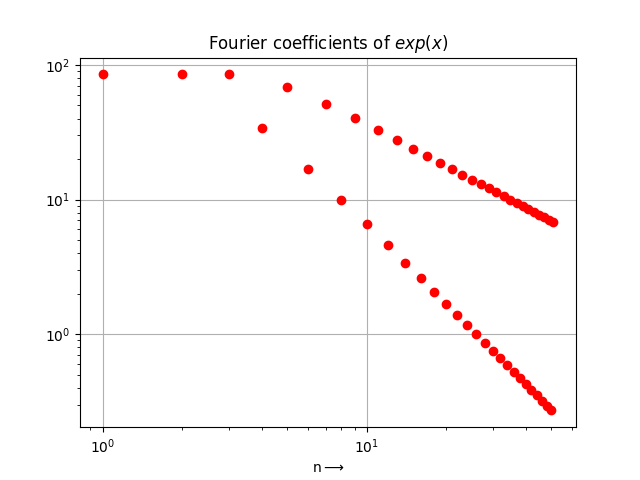
\includegraphics[scale=0.75]{Figure_10.png}
\caption{Coefficients for $exp(x)$ (loglog)}
\end{figure}
\begin{figure}[H]
\centering
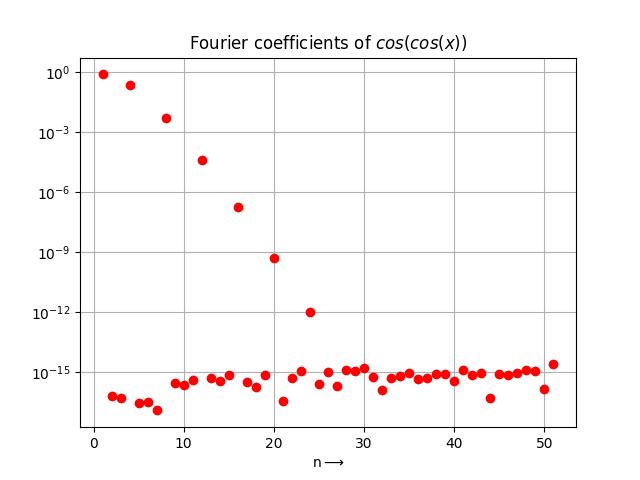
\includegraphics[scale=0.75]{Figure_11.png}
\caption{Coefficients for $cos(cos(x))$ (semilogy)}
\centering
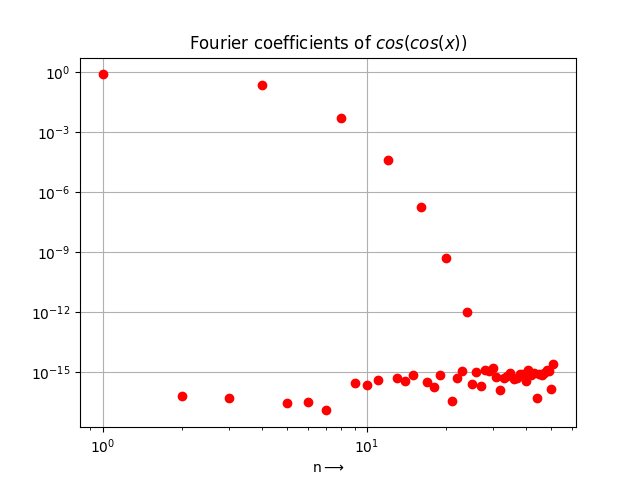
\includegraphics[scale=0.75]{Figure_12.png}
\caption{Coefficients for $cos(cos(x))$ (loglog)}
\end{figure}
 

 
\subsection{Least squares approach}

A finite set of Fourier coeffcients can be found using the \textbf{Least squares approximation} by looking at this as a matrix problem. 400 distinct $x$ values over the interval $[0, 2\pi)$ are considered in this problem. The number of $x$ values can be increased to get better approximations. The resultant matrix equation is
\begin{equation*}
\begin{pmatrix}
1 & cos(x_1) & sin(x_1) & ... & cos(25x_1) & sin(25x_1) \\
... & ... & ... & ... & ... & ... \\
1 & cos(x_{400}) & sin(x_{400}) & ... & cos(25x_{400}) & sin(25x_{400})
\end{pmatrix}
\begin{pmatrix}
a_0 \\
a_1 \\
b_1 \\
... \\
a_{25} \\
b_{25} \\
\end{pmatrix} = 
\begin{pmatrix}
f(x_1) \\
... \\
f(x_{400})
\end{pmatrix}
\end{equation*}
Consider the matrix to be $A$, the coefficients vector be $c$ and the function values vector be $b$. Then the matrix equation is
\begin{equation*}
Ac = b
\end{equation*}
We can use \texttt{lstsq} function from \texttt{scipy.linalg} to approximate the vector $c$. The coefficients for $exp(x)$ and $cos(cos(x))$ can be approximated as shown below
\begin{lstlisting}
x = np.linspace(0, 2*pi, 401)
x = x[:-1]
b1 = e(x)
b2 = coscos(x)
A = np.zeros((400, 51))
A[:,0] = 1
for k in range(1, 26):
    A[:,2*k-1] = np.cos(k*x)
    A[:,2*k] = np.sin(k*x)
c1 = lstsq(A, b1)[0]
c2 = lstsq(A, b2)[0]
\end{lstlisting}

\subsection{Plotting the approximated coefficients}

The \textit{best fit} coefficients for both the functions $exp(x)$ and $cos(cos(s))$ are computed above. They can be plotted along the coefficients compute by direct integration. To differentiate them, green circles are used.
\begin{figure}[H]
\centering
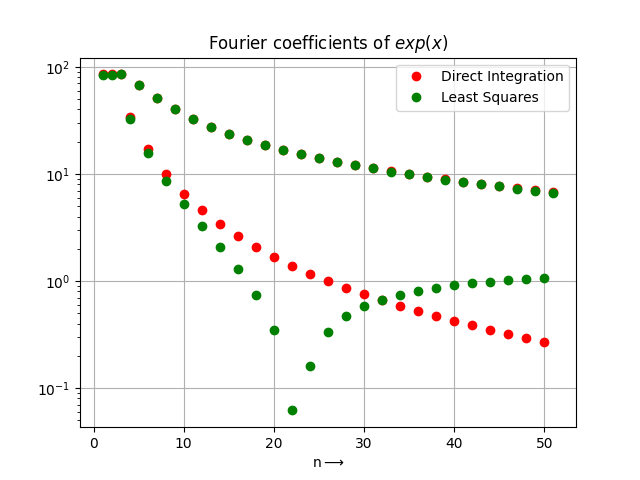
\includegraphics[scale=0.75]{Figure_3.png}
\caption{Coefficients for $exp(x)$ (semilogy)}
\centering
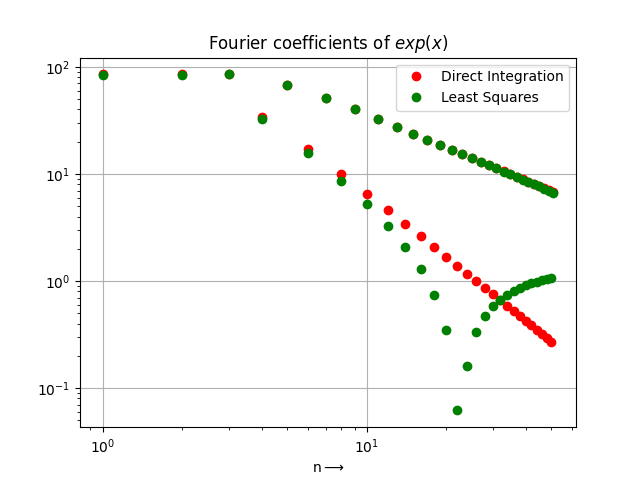
\includegraphics[scale=0.75]{Figure_4.png}
\caption{Coefficients for $exp(x)$ (loglog)}
\end{figure}
\begin{figure}[H]
\centering
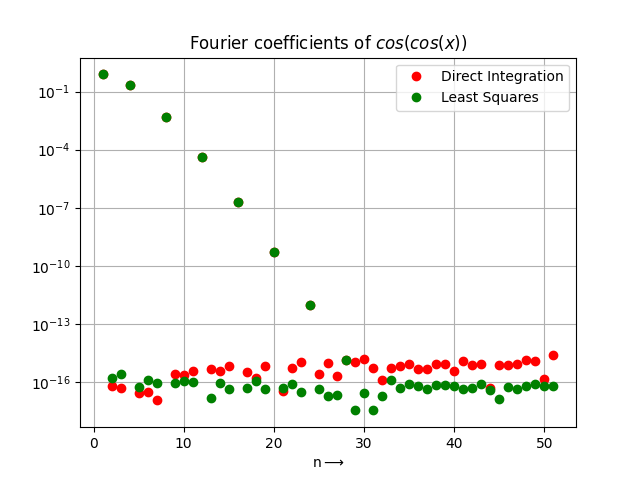
\includegraphics[scale=0.75]{Figure_5.png}
\caption{Coefficients for $cos(cos(x))$ (semilogy)}
\centering
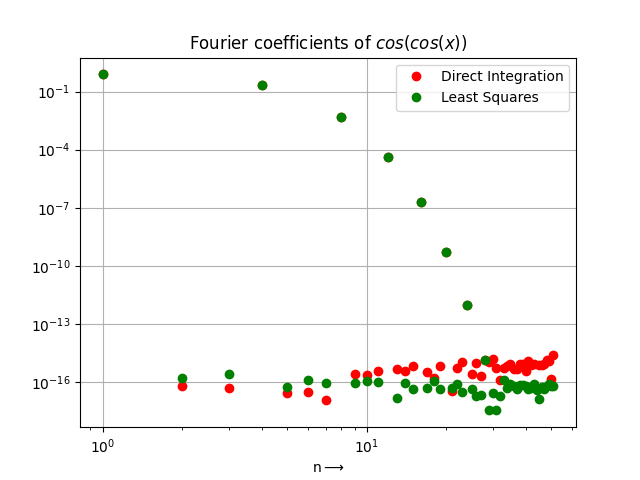
\includegraphics[scale=0.75]{Figure_6.png}
\caption{Coefficients for $cos(cos(x))$ (loglog)}
\end{figure}

\subsection{Comparing the coefficients}

The results from direct integration and least squares approximation agree for $cos(cos(x))$, but there is significant deviation in coefficients of $cos$ terms for $exp(x)$. To find the maximum deviation from actual values, \texttt{np.max} can be used.
\begin{lstlisting}
dev_f1 = np.max(np.abs(c1 - coeffs_f1))
dev_f2 = np.max(np.abs(c2 - coeffs_f2))
\end{lstlisting}
Here, \texttt{c1, c2} are the approximated coefficients and \texttt{coeffs\_f1, coeffs\_f2} are the coefficients from direct integration.
\begin{itemize}
\item The maximum absolute deviation for $exp(x)$ is 1.3327308703353964
\item The maximum absolute deviation for $cos(cos(x))$ is 2.6566469738662125e-15
\end{itemize}

\subsection{Plotting the approximated functions}

The function values for the approxiamted coefficients can be found from the multiplication of matrix $A$ and vector $c$. This will the function values for $x$ over the interval $[0,2\pi)$. For matrix multiplication, \texttt{np.dot} function can be used. The plots of the functions are given below. 
\\ 
High deviation is seen in case of $exp(x)$, but almost no deviation is seen for $cos(cos(x))$. This happens because $2\pi$-periodic extension of $exp(x)$ has a finite discontinuity and the Fourier series deviates from the actual function at the point of discontinuity. This is called \textit{Gibbs phenomenon}. This deviation seen in the plot has very little to do with error in least squares approximation as similar deviation can be seen for direct integration coefficients as well. This does not happen for $cos(cos(s))$ as there is no discontinuity.
\begin{figure}[H]
\centering
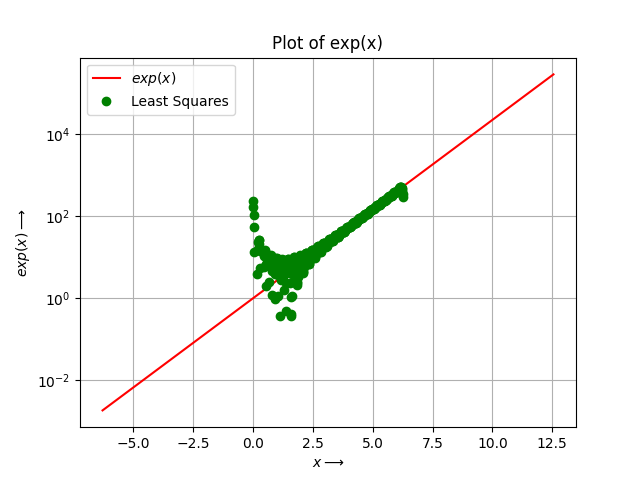
\includegraphics[scale=0.75]{Figure_7.png}
\caption{Approximated $exp(x)$}
\centering
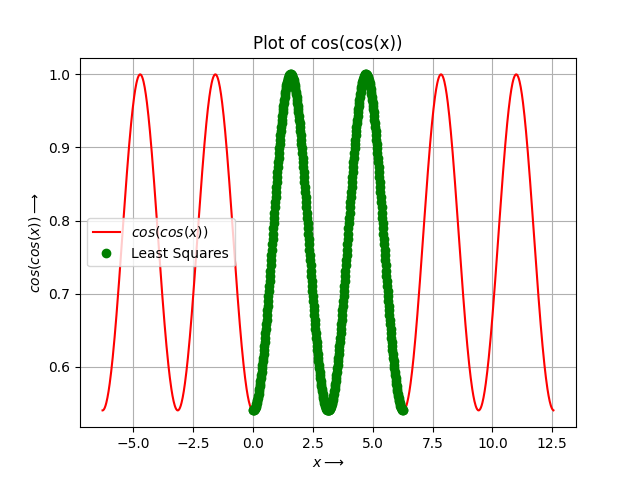
\includegraphics[scale=0.75]{Figure_8.png}
\caption{Approximated $cos(cos(x))$}
\end{figure}

\section{Conclusion}

51 Fourier coefficients of $exp(x)$ and $cos(cos(x))$ are computed by integration and their variation with $n$ is observed. It was seen that even functions have sine-coefficients as 0 in Fourier series. The coeffcients are also approximated using \textit{least squares method} and the deviation from integration coefficients was observed.  The peculiar deviation of Fourier series from actual function after jump discontinuity, called \textit{Gibbs phenomenon}, was observed.

\end{document} 